\begin{document}
\section{Pictures}
\begin{figure}
  \centering
  \begin{tikzpicture}[scale=0.8, every node/.style={draw}]
    \node (a) at (0,0) {A}; % a comment with \end{tikzpicture} in it
    \node (b) at (2,0) {B};
    \draw[->] (a) -- (b);
  \end{tikzpicture}
  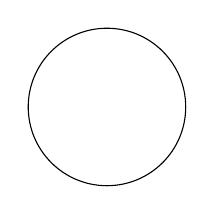
\begin{tikzpicture}
    \draw (0,0) circle (1);
  \end{tikzpicture}
  \caption{Two diagrams in one float.}
  \label{fig:two}
\end{figure}

\begin{figure}
  \begin{forest}
    [S [NP [she]] [VP [runs]]]
  \end{forest}
  \caption{A parse tree.}\label{fig:tree}
\end{figure}

\begin{figure*}
  \begin{subfigure}{0.5\textwidth}
    \begin{circuitikz} \draw (0,0) to[R] (2,0); \end{circuitikz}
    \caption{A resistor.}\label{fig:r}
  \end{subfigure}
  \begin{subfigure}{0.5\textwidth}
    \begin{picture}(100,50)
      \put(0,0){\line(1,0){100}}
    \end{picture}
    \caption{A line.}
  \end{subfigure}
  \caption{Circuit and line.}
\end{figure*}

\begin{table}
  \caption{A table drawn as a picture.}\label{tab:pic}
  \begin{pgfpicture}
    \pgfpathmoveto{\pgfpointorigin}
  \end{pgfpicture}
\end{table}

Figures~\ref{fig:two}, \ref{fig:tree} and \ref{fig:r}; Table~\ref{tab:pic}.
\end{document}
